% \vspace{-1.5cm}
\section{MAMBO-G: Magnitude-Aware Mitigation}
\subsection{The Risk of Zero-SNR Guidance}
Rectified Flow \cite{liu2022flow} typically initializes sampling from a pure noise state $\x_1\sim\mathcal{N}(\Zero, \One)$ at time $t=1$ to get an example $x_0$ from the original data distribution $\Data$. The velocity field guides the noise $\x_1$ towards the data $\x_0$.
\begin{equation}
    \vel(\x_t, t, c) = \E_{\x_0\sim \Data, \x_1\sim\mathcal N(\Zero, \One)}\left[\left. \x_0 - \x_1 \,\right|\, \x_t, c \right],
\end{equation}
where $\x_t$ is the intermediate state. We denote the conditional velocity as $\vel(\x_t, t, c)$ and the unconditional one as $\vel(\x_t, t, \varnothing)$. The classifier-free guidance substitutes $\vel(\x_t, t, c)$ with $\tilde\vel(\x_t, t, c)$ during sampling, which is defined as:
\begin{equation}
\begin{aligned}
    \tilde\vel(\x_t, t, c) &\\:= w&\cdot(\vel(\x_t, t, c) - \vel(\x_t,t,\varnothing)) + \vel(\x_t,t,\varnothing),
\end{aligned}
\end{equation}
where $w$ is the guidance scale and the \textbf{guidance update} $\Delta\vel(x_t,t,c):=\vel(\x_t, t, c) - \vel(\x_t,t,\varnothing)$.

At the initialization step ($t=1$), the input $\x_1$ is pure noise and statistically independent of the data $\x_0$. Consequently, $\x_1$ provides no spatial or semantic cues about the target image. The model prediction for $\hat\x_0=\E\left[\x_0|\x_t,c\right]$ thus reduces to the conditional expectation that only depends on the text prompt $c$:
\begin{equation}
\begin{aligned}
    \mean_{\cond}&:= \E\left[\left.\x_0 \,\right|\x_1, ~c~ \right]= \E\left[\left.\x_0 \,\right|~c~ \right], \\
    \mean_{\uncond}&:= \E\left[\left.\x_0 \,\right|\x_1, ~c~ \right]= \E\left[\left.\x_0 \,\right|\, \varnothing~ \right].
\end{aligned}
\end{equation}
At this initial step, the guidance update $\Delta \vel(\x_1,1,c)$ reduces to a constant offset:
\begin{equation}
\begin{aligned}
    \Delta \vel_c &= \vel(\x_1, 1, c) - \vel(\x_1, 1, \varnothing) \\
    &=\E\left[\x_0-\x_1|\x_1,c\right] - \E\left[\x_0-\x_1|\x_1,\varnothing\right]\\
    &=(\mean_{\cond} - \x_1) - (\mean_{\uncond} - \x_1)\\
    &= \mean_{\cond} - \mean_{\uncond}.
\end{aligned}
\end{equation}

\begin{figure}[t]
    \centering
    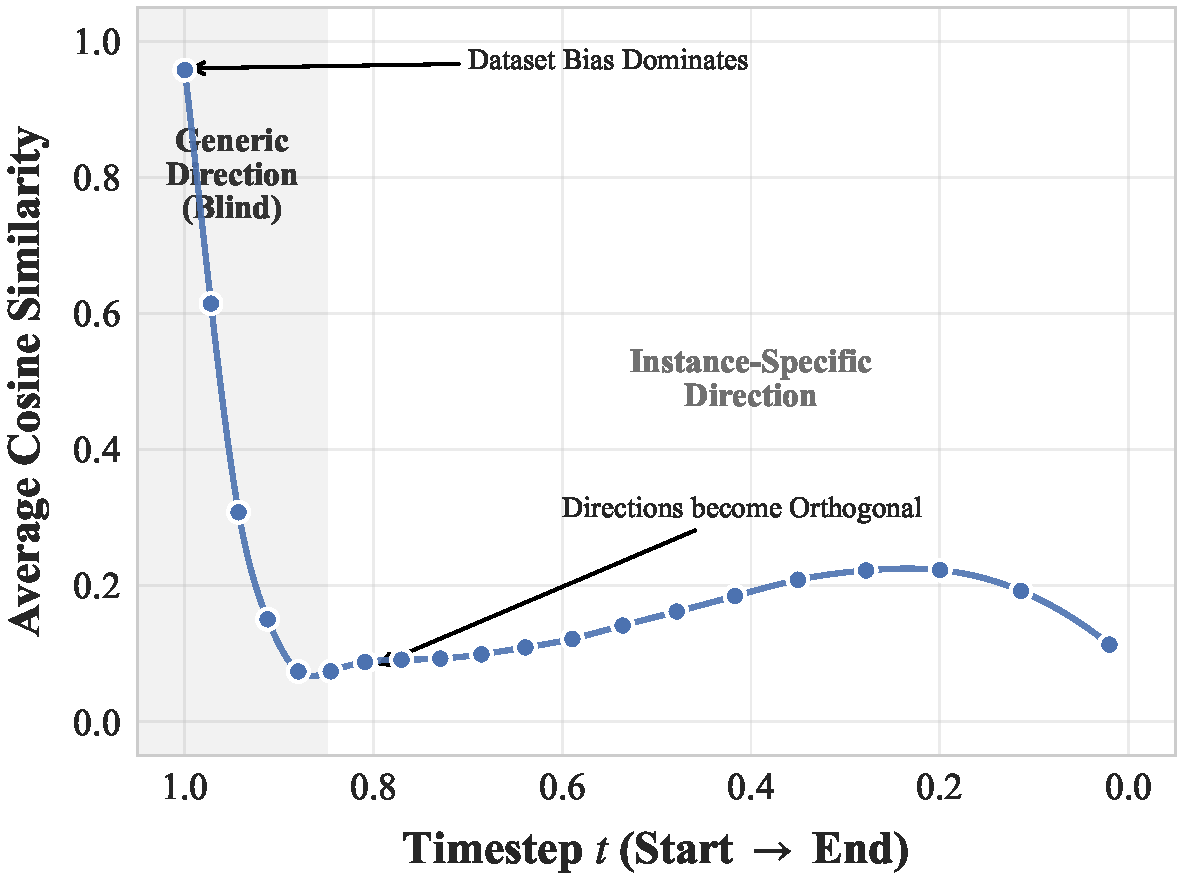
\includegraphics[width=0.48\textwidth]{fig_tab/cosine_similarity_analysis.pdf}
    \vspace{-0.1in} 
    % \caption{\textbf{Collapse of Guidance Directions at Initialization.} We measure the cosine similarity of guidance update vectors ($\Delta \vel$) across different random noise seeds for a fixed prompt throughout the sampling process. At $t=1.0$ (initialization), the updates are nearly identical (Similarity $\approx 1.0$), indicating that the guidance direction is generic and independent of the specific noise instance. As sampling progresses ($t < 0.8$), the directions rapidly diverge (Similarity $\to 0$), becoming instance-specific. This observation motivates \mtdbk to dampen the guidance scale specifically in the high-similarity, generic regime.}
    \caption{\textbf{Collapse of Guidance Directions at Initialization.} We analyze the cosine similarity of guidance updates ($\Delta \vel$) across different noise seeds for a fixed prompt. At $t=1.0$, similarity $\approx 1.0$, indicating a generic direction independent of specific noise. As $t$ decreases ($t < 0.8$), updates rapidly diverge and become instance-specific. This observation motivates \mtdbk to dampen the guidance scale specifically in this high-similarity, generic regime.}
    \label{fig:cosine_sim}
    \vspace{-0.15in}
\end{figure}

\begin{figure}[t]
    \centering
    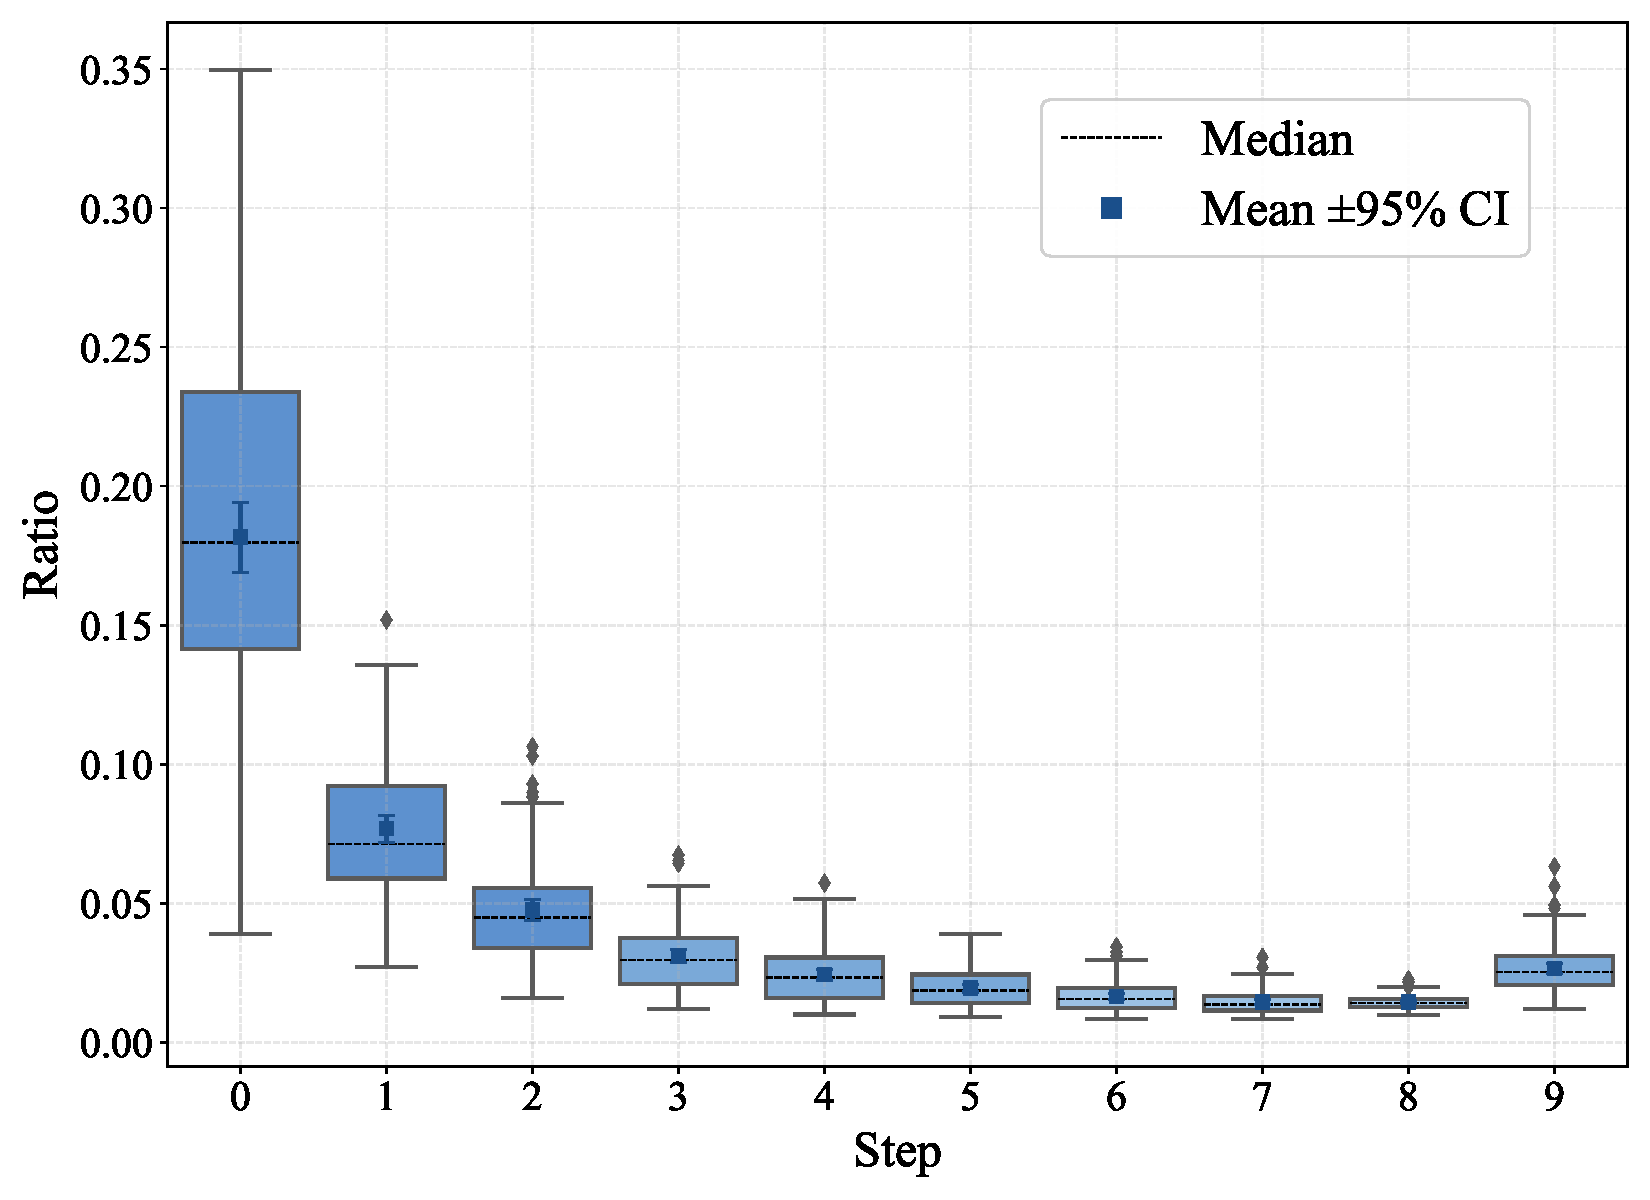
\includegraphics[width=0.47\textwidth]{fig_tab/ratio_distribution_by_step.pdf} 
    \vspace{-0.1in} 
    % \caption{\textbf{Dynamics of the ratio during sampling}. The Ratio starts high, which indicates strong conditional influence, but rapidly decays within a few steps and stabilizes.}
    \caption{\textbf{Dynamics of the ratio during sampling.} We monitor the evolution of the relative guidance strength $r_t$ throughout the sampling process. The ratio starts at a high peak, reflecting a strong conditional influence that can lead to early-stage instability if left unregulated. It then rapidly decays and stabilizes within a few sampling steps. This empirical trend identifies the initial phase as a critical regime where guidance damping mechanism is most necessary.}
    \label{fig:ratio_distribution_step}
    \vspace{-0.15in}
\end{figure}
This difference $\Delta \vel$ is a \textbf{generic direction} based on dataset statistics. \textbf{It is independent of the sampled noise $\x_1$}.

To understand the guidance behavior at initialization, we analyze the consistency of guidance updates $\Delta \vel$ across different random noise samples for fixed prompts. As shown in \Cref{fig:cosine_sim}, the cosine similarity is approximately \textbf{1.0} at $t=1$. This confirms that the initial guidance is a \textbf{generic direction} determined solely by the prompt, independent of the specific noise $\x_1$.

Applying a large guidance scale to this generic direction is risky. Since the update ignores the specific noise structure, a strong force can drive the trajectory away from the valid data distribution. However, this state is temporary. The similarity drops quickly as sampling continues ($t < 0.8$), and the guidance becomes \textbf{instance-specific}. This motivates \mtdbk: we reduce the guidance scale during this initial generic phase to prevent instability, then boost it to further enhance the guidance effect as the image structure forms.


\subsection{Quantifying the Relative Guidance Strength}
Although the guidance direction $\Delta \vel$ at $t=1$ is independent of $x_1$, the magnitude of the model's conditional velocity $\vel_{\cond}$ is highly instance-dependent. To quantify the relative strength of the guidance update, we define the ratio $r_t$:
\begin{equation}
    r_t = \frac{\norm[2]{\vel(\x_t, t, c) - \vel(\x_t, t, \varnothing)}}{\norm[2]{\vel(\x_t, t, \varnothing)}}.
    \label{eq:ratio}
\end{equation}

% From a statistical perspective, $r_t$ functions as the coefficient of variation (CV) of the velocity field. 
From a statistical perspective, $r_t$ provides an \textbf{instance-specific estimation of the relative fluctuation} within the velocity field, functionally analogous to the coefficient of variation (CV). 
This interpretation holds because the unconditional velocity $\vel(\x_t, t, \varnothing)$ approximates the expected trajectory marginalized over the distribution of prompts, while the conditional velocity $\vel(\x_t, t, c)$ acts as a specific realization. 

Intuitively, a high coefficient of variation indicates large relative fluctuations in the guidance-induced discrepancy, reflecting an unstable conditional influence. Such excessive deviation suggests that the conflict between the prompt and the intrinsic image structure is severe, potentially leading to generation artifacts. Therefore, samples with excessively high $r_t$ are risky outliers that require mitigation. 

% This ratio serves as a normalized metric of guidance intensity, comparing the conditional deviation against the baseline unconditional velocity.

% From a statistical perspective, $r_t$ functions as the coefficient of variation for the velocity field. Since the unconditional velocity $\vel_{\uncond}$ approximates the expected trajectory towards the data manifold ($\vel_{\uncond} \approx \E_c[\vel_{\cond}]$), a large $r_t$ implies a significant deviation from the mean behavior. Formally, by applying Chebyshev's inequality, we can upper bound the probability of observing a large relative deviation $r_t \ge \lambda$:
% \begin{equation}
% \begin{aligned}
%     P(r_t \ge \lambda) &= P\left( \|\vel(\x_t, t, c) - \vel(\x_t, t, \varnothing)\|_2 \ge \lambda \|\vel(\x_t, t, \varnothing)\|_2 \right) \\
%     &\le \frac{\E_c[\|\vel(\x_t, t, c) - \vel(\x_t, t, \varnothing)\|_2^2]}{\lambda^2 \| \vel(\x_t, t, \varnothing)\|_2^2}.
% \end{aligned}
% \end{equation}
% This inequality suggests that states with excessively high $r_t$ are statistical outliers within the valid velocity distribution learnt by the model. Relying on such atypical updates is inherently risky, as they likely correspond to unstable regions where the guidance force overwhelms the data manifold's structure.

Empirically, as shown in \Cref{fig:ratio_distribution_step}, this risk is most pronounced during the initialization phase ($t \to 1$), where $r_t$ reaches its peak. This high-ratio phase coincides with the generic direction regime (\Cref{fig:cosine_sim}), where the guidance direction is not yet adapted to the specific noise instance. Consequently, applying a large guidance scale when $r_t$ is high risks amplifying generic, coarse features in an uncontrolled manner, rather than refining the image structure. Thus, $r_t$ serves as a robust indicator for potential instability, necessitating a damping mechanism to prevent trajectory collapse.

\begin{figure}[t]
    \centering
    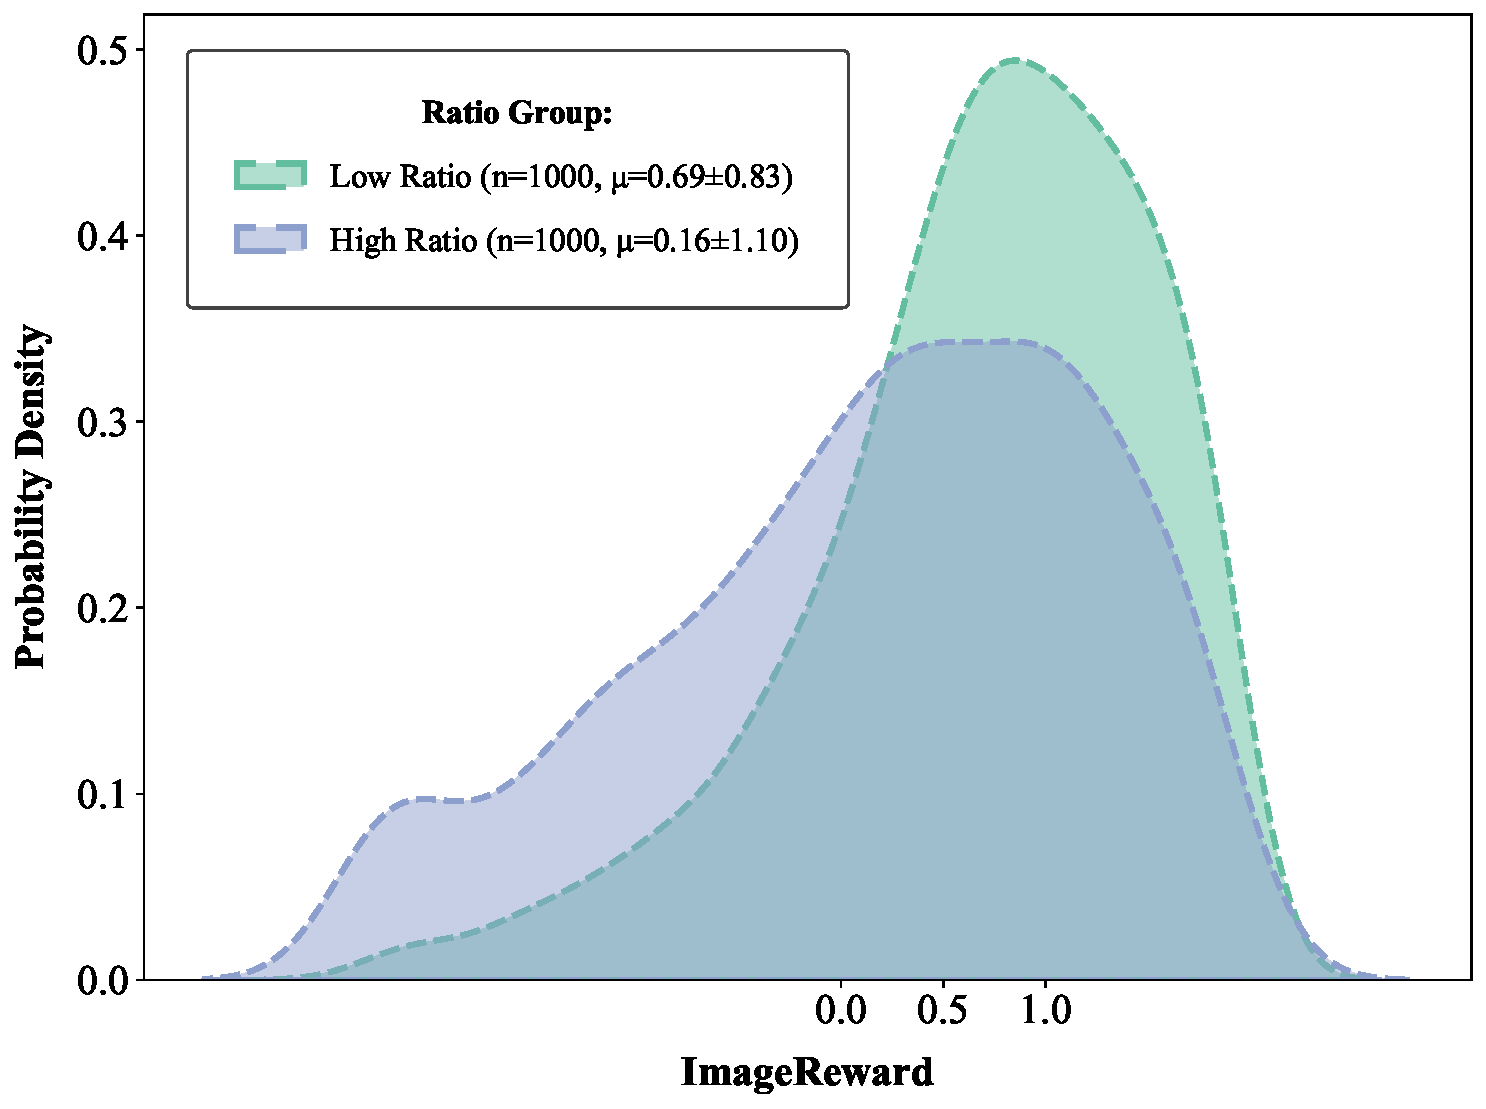
\includegraphics[width=0.47\textwidth]{fig_tab/professional_kde.pdf} 
    \vspace{-0.1in} 
    % \caption{\textbf{Probability density of ImageReward scores across different Ratio groups.}
    % KDE plots of ImageReward for low-Ratio  versus high- Ratio  samples collected at the first sampling step}
    \caption{\textbf{Probability density of ImageReward scores across different Ratio groups.} We present KDE plots comparing ImageReward scores for low-ratio versus high-ratio samples at the first sampling step. The results show that lower initial ratios yield significantly higher quality, validating the ratio as a robust indicator for predicting sampling stability.}
    \label{fig:high_ratio_vs_low_ratio}
    \vspace{-0.15in}
\end{figure}

\begin{figure}[t]
    \centering
    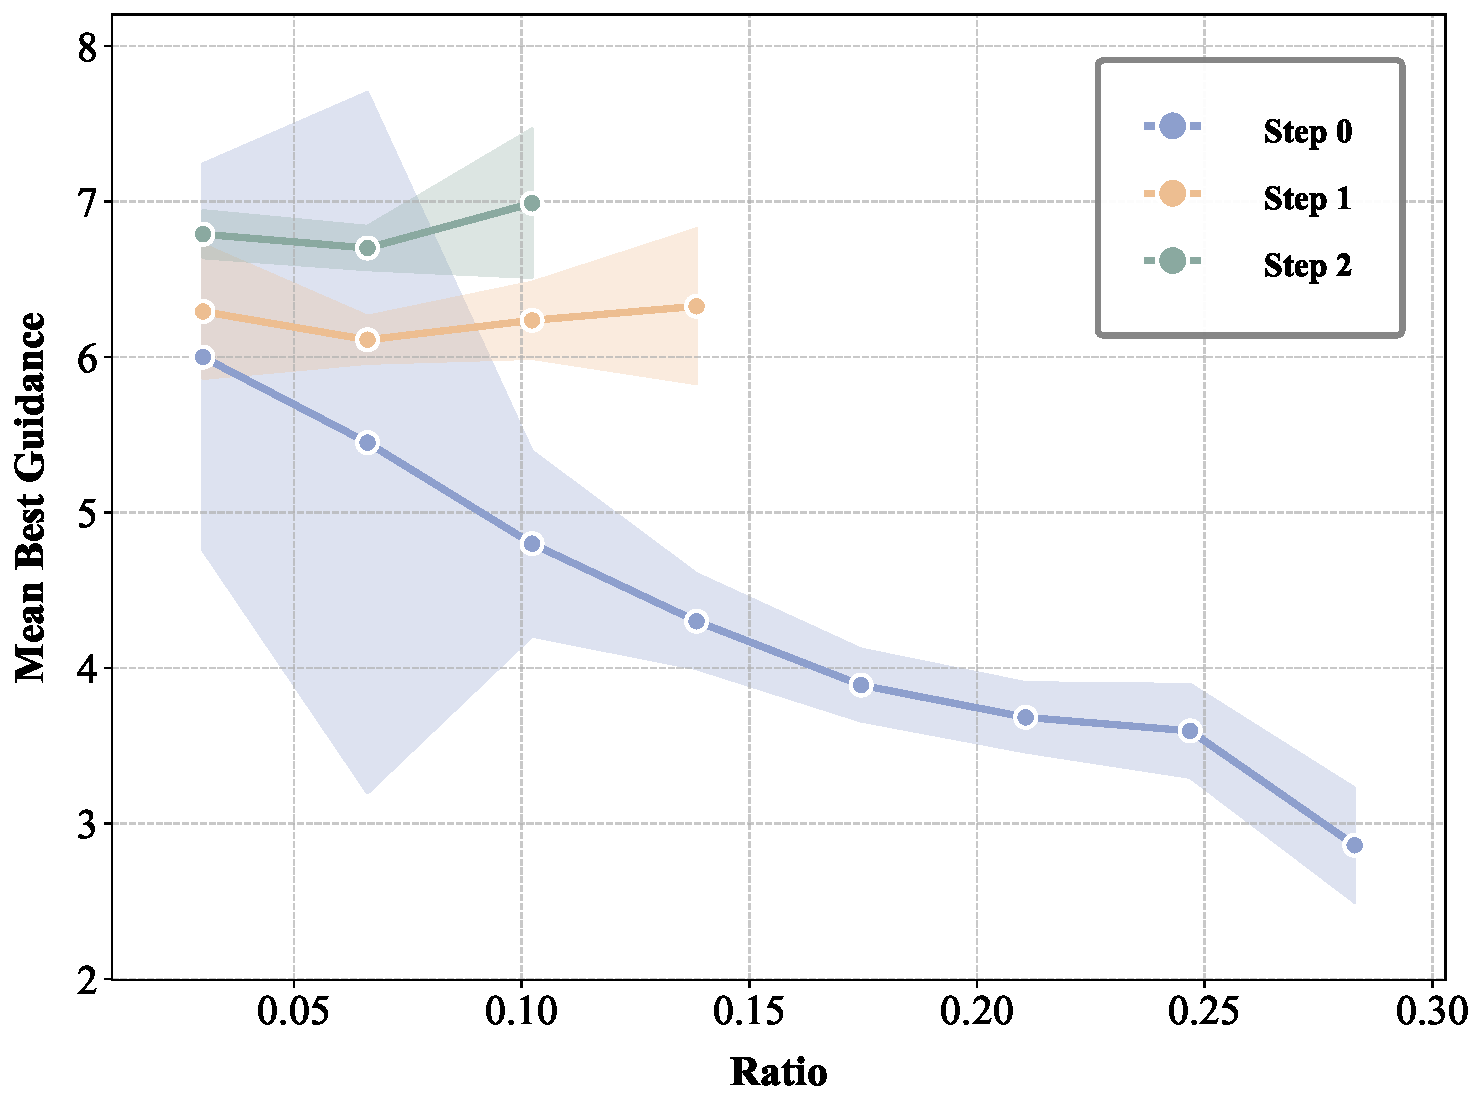
\includegraphics[width=0.48\textwidth]{fig_tab/ratio_vs_guidance_ci.pdf}
    \vspace{-0.1in} 
    % \caption{\textbf{Optimal Guidance Scale vs. Ratio.} We perform a greedy search to identify the optimal guidance scale that maximizes ImageReward for varying ratio values. The scatter plot illustrates that the optimal scale decreases as the ratio increases, exhibiting a trend that aligns well with an exponential decay. This observation supports our use of an exponential function to model the damping schedule.}
    \caption{\textbf{Optimal Guidance Scale vs. Ratio.} We perform a greedy search to identify the optimal guidance scale maximizing ImageReward for various ratios. The results illustrate that the optimal scale decreases as the ratio increases, exhibiting an exponential decay. This trend directly motivates our use of an exponential damping function.}
    \label{fig:ratio_guidance_fit}
    \vspace{-0.15in}
\end{figure}

\subsection{Empirical Dynamics and Sample Heterogeneity}
Our observations align with \citet{lin2024common} regarding the instability of zero-SNR sampling. To further investigate this, we designed an ablation study on SD3.5. We used 100 prompts, with 20 seeds corresponding to each prompt. The ratio value at the first step was calculated for each of these 20 seeds per prompt, allowing us to divide them equally into high-ratio and low-ratio groups. Sampling was then performed using a default guidance scale of 7. The results, presented in \Cref{fig:high_ratio_vs_low_ratio}, demonstrate that the quality of the high-ratio group was significantly lower than that of the low-ratio group. This experimentally suggests that the ratio can serve as an effective metric for modeling sampling stability. Notably, we observe considerable variance in ratio values across different samples, even at the same timestep $t$. Standard dynamic guidance strategies rely on time-dependent schedules $w(t)$. However, as shown in our analysis, the ratio $r_t$ varies significantly across samples even at the same timestep. A purely time-based schedule $w(t)$ ignores this heterogeneity, failing to selectively mitigate the instability of high-ratio outliers. This observation provides empirical support for our approach of modeling guidance based on the ratio $w(r_t)$ rather than time alone.

\begin{figure*}[t]
    \centering
    \begin{subfigure}{0.49\textwidth}
        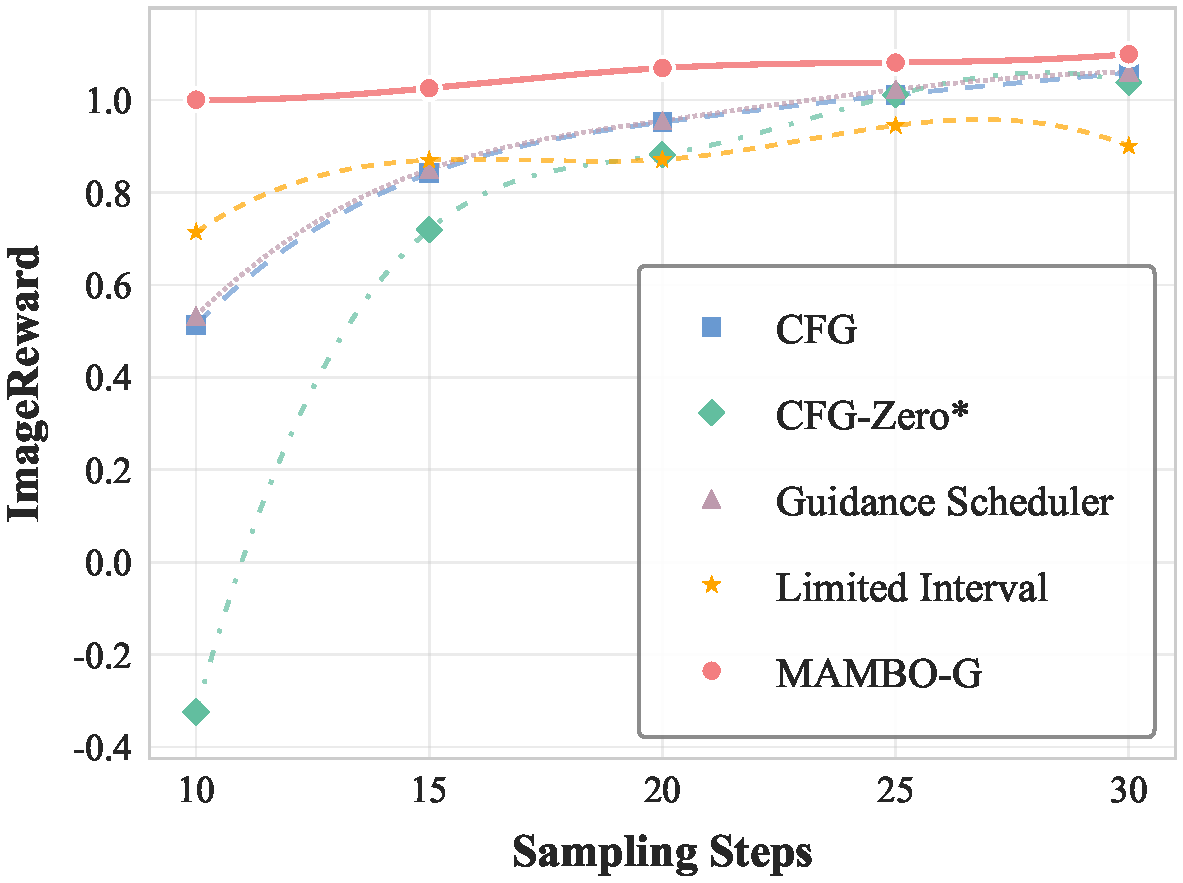
\includegraphics[width=\linewidth]{fig_tab/SD35_ImageReward_comparison.pdf}
        \captionsetup{justification=justified, singlelinecheck=true}
        \caption{SD3.5, ImageReward.}
        \label{fig:sub1_1}
    \end{subfigure}
    \hfill
    \begin{subfigure}{0.49\textwidth} 
        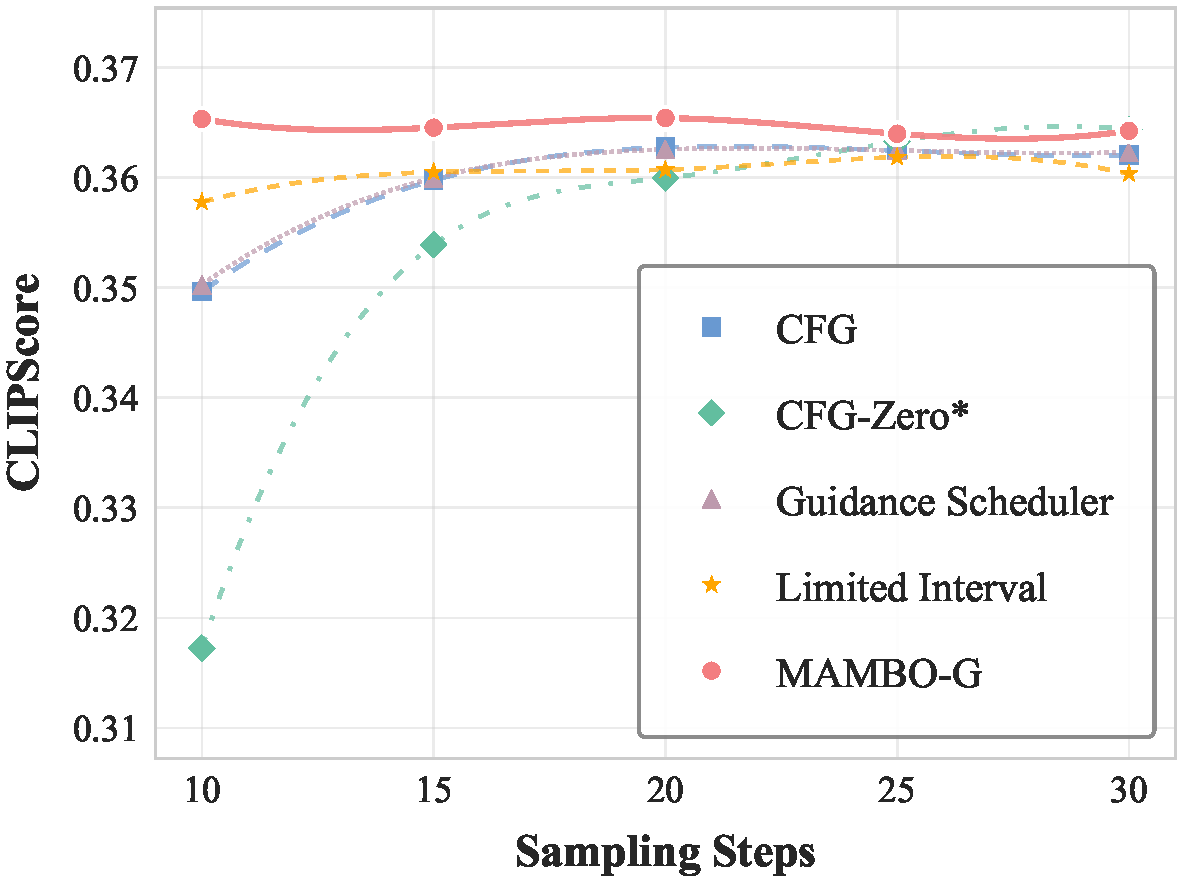
\includegraphics[width=\linewidth]{fig_tab/SD35_CLIPScore_comparison.pdf}
        \captionsetup{justification=justified, singlelinecheck=true}
        \caption{SD3.5, CLIPScore.}
        \label{fig:sub2_1}
    \end{subfigure}
    \begin{subfigure}{0.49\textwidth}
        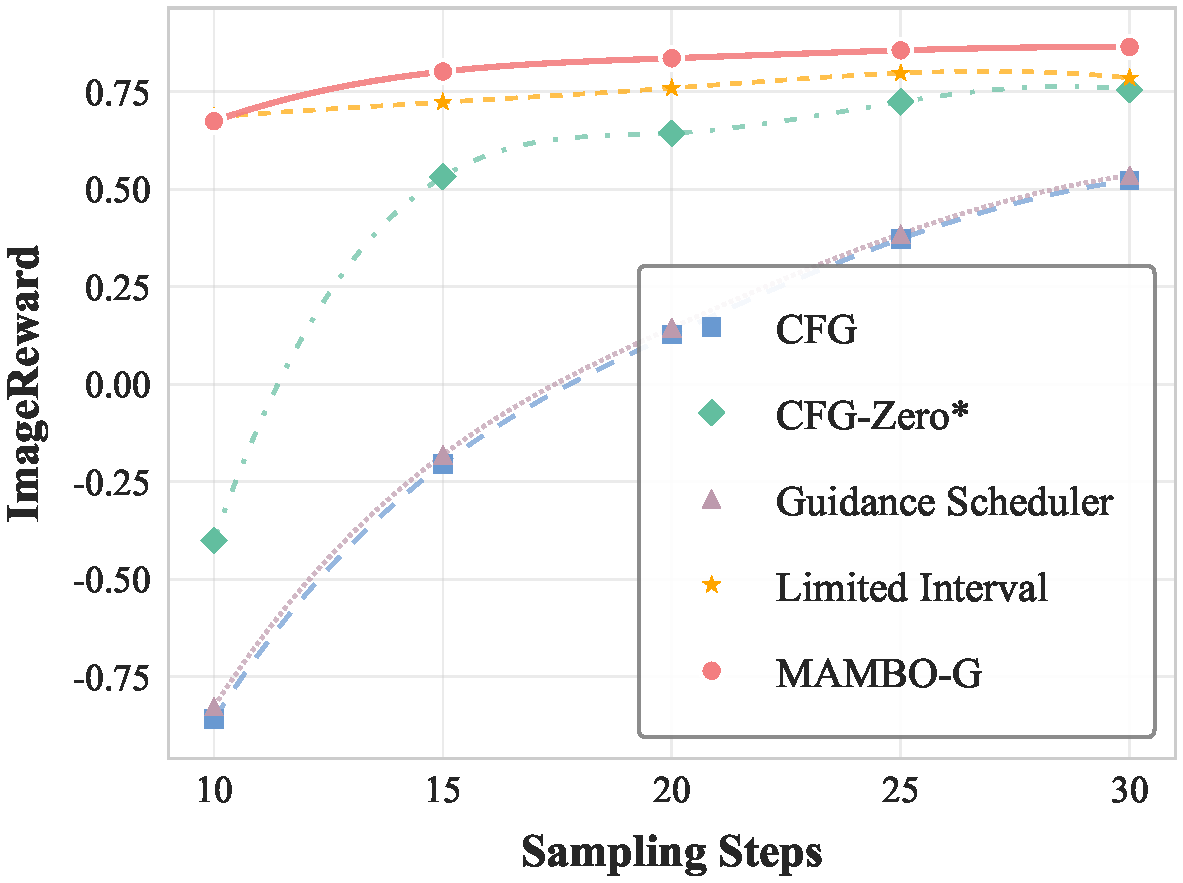
\includegraphics[width=\linewidth]{fig_tab/LUMINA_ImageReward_comparison.pdf}
        \captionsetup{justification=justified, singlelinecheck=true}
        \caption{Lumina, ImageReward.}
        \label{fig:sub1_2}
    \end{subfigure}
    \hfill
    \begin{subfigure}{0.49\textwidth} 
        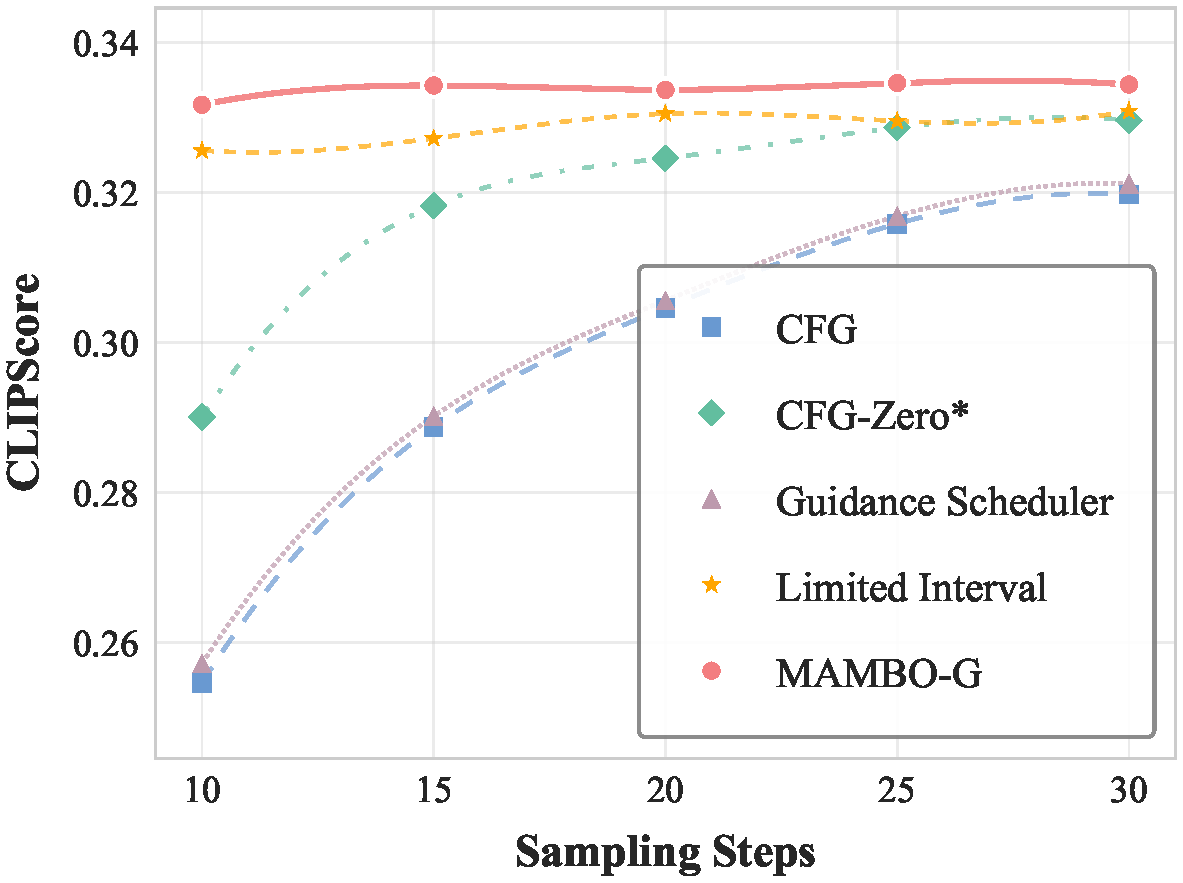
\includegraphics[width=\linewidth]{fig_tab/LUMINA_CLIPScore_comparison.pdf}
        \captionsetup{justification=justified, singlelinecheck=true}
        \caption{Lumina, CLIPScore.}
        \label{fig:sub2_2}
    \end{subfigure}
    
    \captionsetup{justification=justified, singlelinecheck=false}
    \caption{\textbf{Quantitative results of comparative analysis with other baselines in text-to-image generation measured by ImageReward and CLIPScore.} Here, \textbf{Guidance Scheduler} refers to ~\citet{xianalysis} and \textbf{Limited Interval} refers to ~\citet{kynkaanniemi2024applying}. The results demonstrate \methodabbr's remarkable superiority over others in low-step generation, achieving the quality of $30$-step generation of CFG in only \textbf{$\mathbf{10}$ steps.}}
    \label{fig:txt2img_compare}
\end{figure*}
\label{sec:exp}

\subsection{MAMBO-G: Adaptive Damping Strategy}

Building on the statistical insight that updates with high $r_t$ represent outliers (Eq.~\ref{eq:ratio}), we formulate the damping function $w(r_t)$ to mitigate the risk of these deviations. Since high-$r_t$ updates likely exceed the valid velocity distribution, relying on them with a strong guidance scale typically leads to trajectory collapse or artifacts.

To determine the optimal suppression schedule, we turn to the empirical evidence. By performing a controlled grid search for the maximum effective guidance scale across varying $r_t$ (see \Cref{alg:greedy_search}), we derive an empirical reference curve (visualized in \Cref{fig:ratio_guidance_fit}). We observe that the model's tolerance for strong guidance does not decay linearly, but drops sharply as the update becomes more disproportionate. To strictly align the guidance strength with this safe regime, we fit the stability boundary with an exponential decay function:
\begin{equation}
    w(r_t) = 1 + (w_{\max} - 1) \cdot \exp(-\alpha r_t).
\end{equation}
Here, $w_{\max}$ represents the maximum allowable guidance scale, and $\alpha > 0$ is a hyperparameter calibrated to the decay rate of the reference curve.

This formulation acts as a continuous, magnitude-aware filter. It permits aggressive boosting when the conditional update is statistically normal ($r_t \to 0$) but applies exponentially stronger damping as $r_t$ increases. By dynamically suppressing the specific "outlier" updates identified by $r_t$, \mtdbk prevents the amplification of unstable directions while retaining the benefits of high guidance in safe regions.

\begin{figure*}[t]
    \centering
    \begin{subfigure}{0.49\textwidth}
        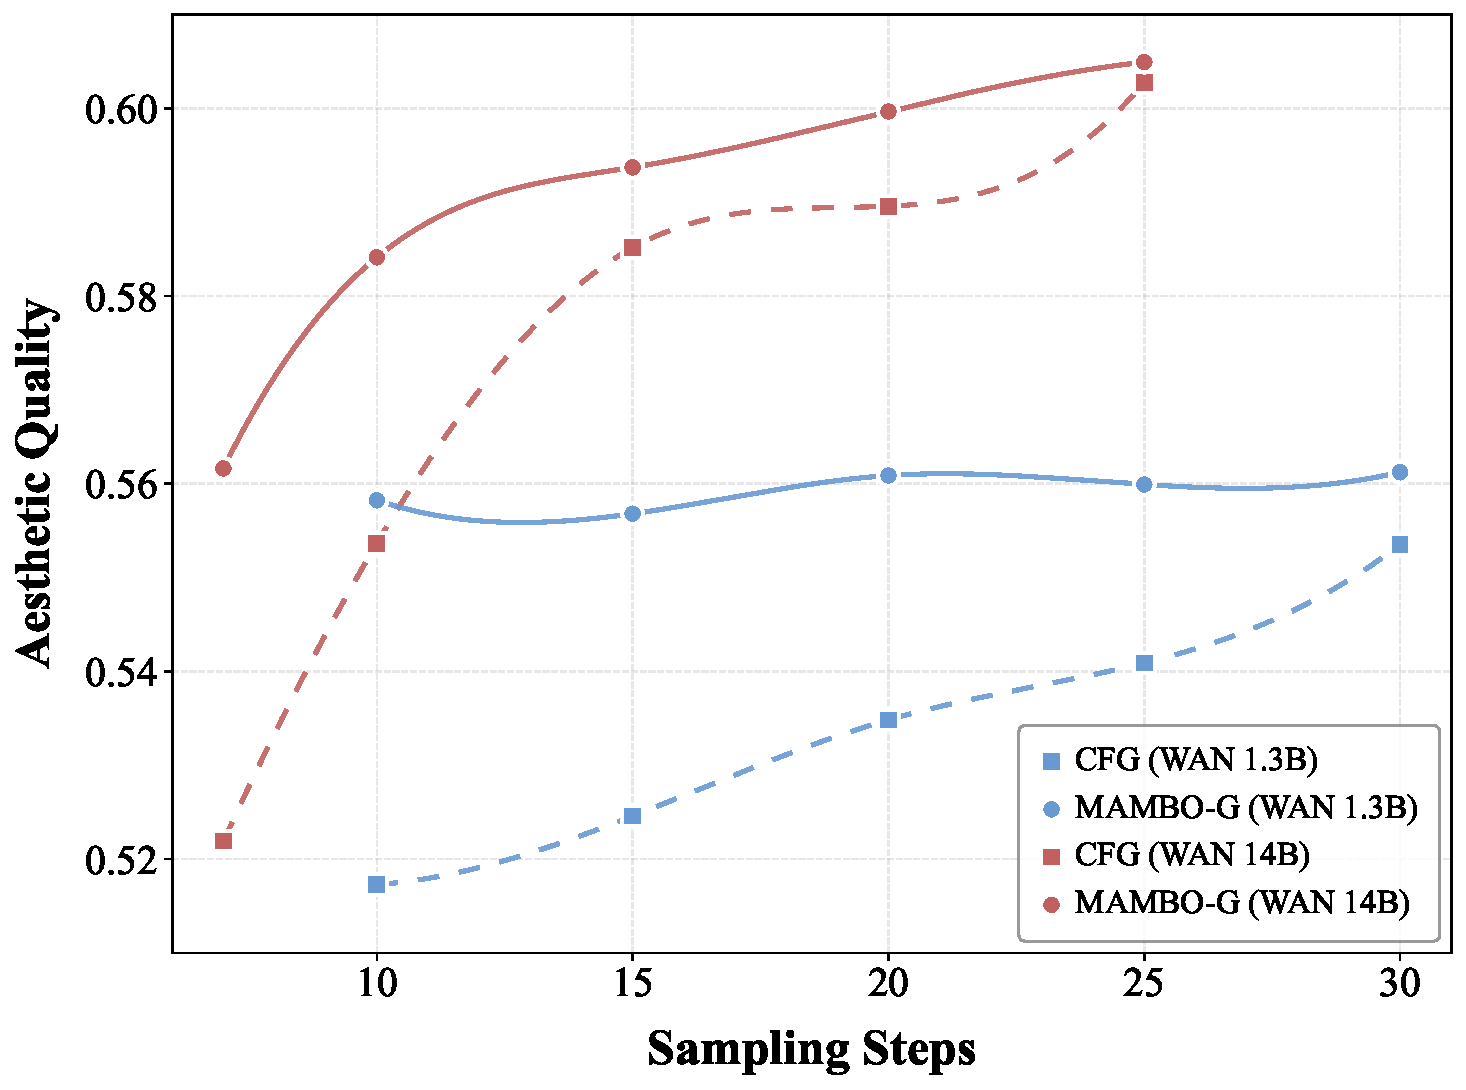
\includegraphics[width=\linewidth]{fig_tab/UniPC_Aesthetic_Quality_comparison.pdf}
        \captionsetup{justification=justified, singlelinecheck=true}
        \caption{vBench: Imaging Quality.}
        \label{fig:sub1_1}
    \end{subfigure}
    \hfill
    \begin{subfigure}{0.49\textwidth} 
        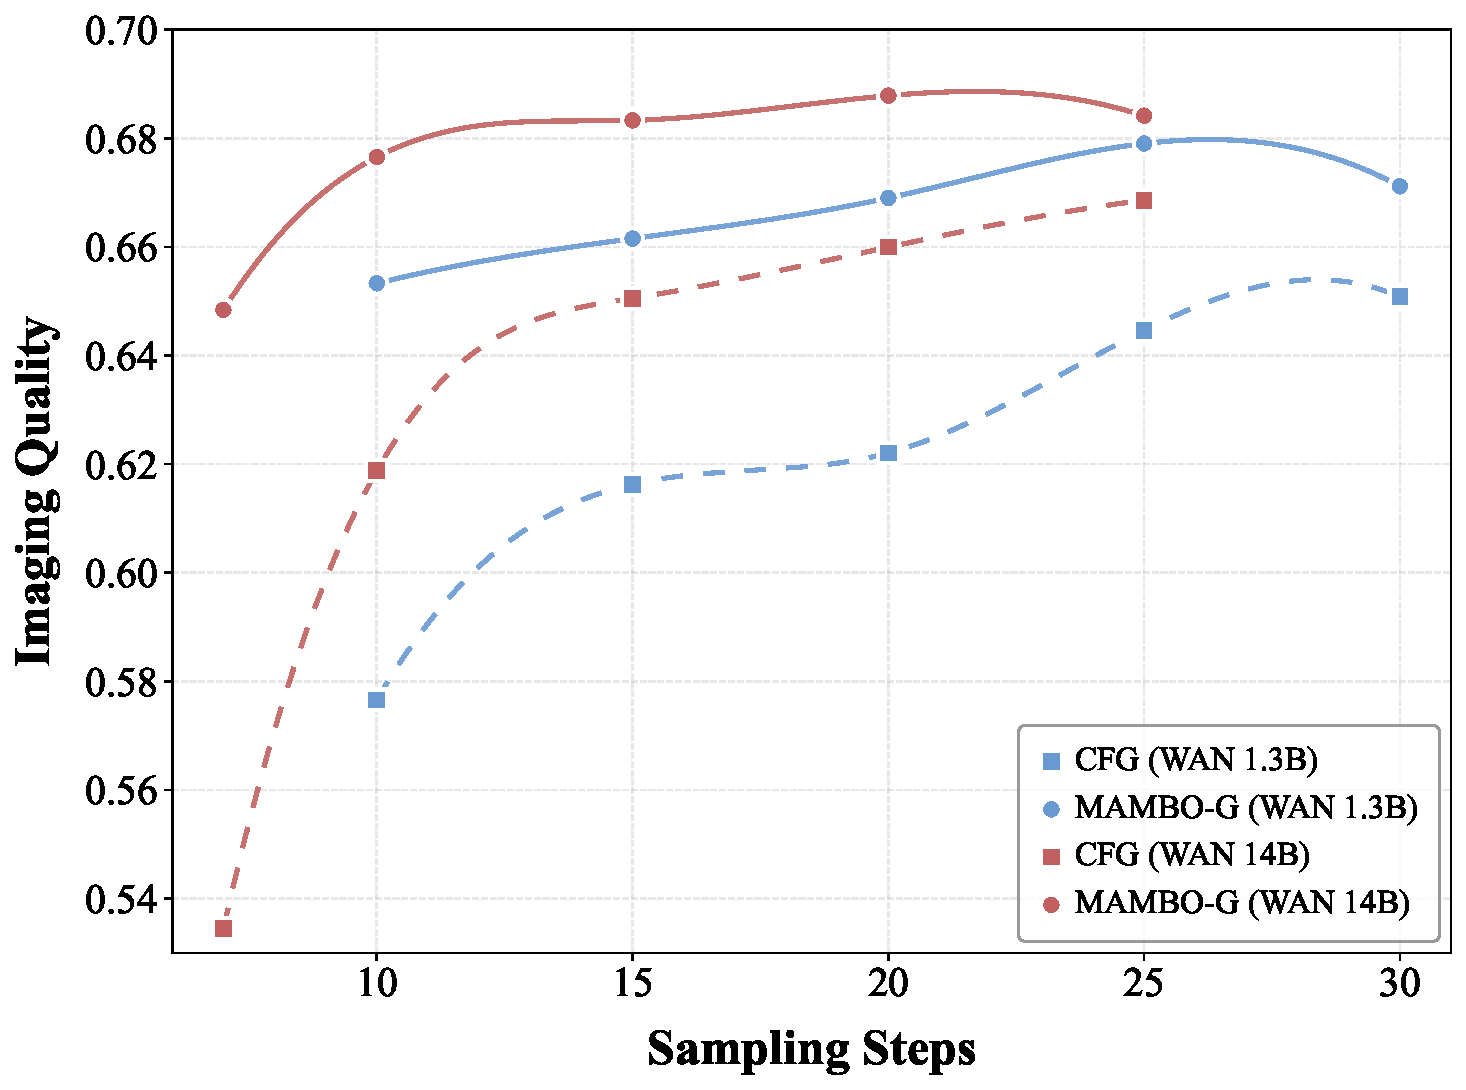
\includegraphics[width=\linewidth]{fig_tab/UniPC_Imaging_Quality_comparison.pdf}
        \captionsetup{justification=justified, singlelinecheck=true}
        \caption{vBench: Aesthetic Quality.}
        \label{fig:sub2_1}
    \end{subfigure}
    \captionsetup{justification=justified, singlelinecheck=false}
    \caption{\textbf{Quantitative results of text-to-video generation, comparing \textbf{CFG and \mtdbk} under vBench.} The results strongly validate the effectiveness of \mtdbk on video generations, even overtaking CFG-Wan 14B just on Wan 1.3B.}
    \label{fig:txt2video_compare}
\end{figure*}
\label{sec:exp}